\documentclass[conference]{IEEEtran}
\IEEEoverridecommandlockouts
% The preceding line is only needed to identify funding in the first footnote. If that is unneeded, please comment it out.
%\usepackage{cite}
\usepackage{amsmath,amssymb,amsfonts}
\usepackage{algorithmic}
\usepackage{graphicx}
\usepackage{textcomp}
\usepackage{xcolor}
\usepackage{hyperref}
\usepackage{biblatex}
\usepackage{soul}
\usepackage{balance}
\usepackage{combelow}
\usepackage[normalem]{ulem}
\usepackage{multirow}
\addbibresource{bibliography.bib}

\def\BibTeX{{\rm B\kern-.05em{\sc i\kern-.025em b}\kern-.08em
    T\kern-.1667em\lower.7ex\hbox{E}\kern-.125emX}}
\begin{document}

\title{UOLO: A Multitask U-Net YOLO Hybrid Model for Railway Scene Understanding.}
% https://www.overleaf.com/project/625ad1dfab03cbf3da656f9b

\author{\IEEEauthorblockN{Alexandru Manole, Laura-Silvia Dio\cb{s}an}
\IEEEauthorblockA{\textit{Department of Computer-Science} \\
\textit{Faculty of Mathematics and Computer Science}\\
\textit{Babeș-Bolyai University}\\
Cluj-Napoca, Romania\\
alexandru.manole@ubbcluj.ro, laura.diosan@ubbcluj.ro}
}

\maketitle

\begin{abstract}
Extracting essential information including the topological structure of  rail-tracks, the\ position of switches and their current state can increase safety by reducing human error, while also boosting the efficiency of rail transportation. Despite the impressive advancements in the field of autonomous driving, computer vision approaches in the rail domain are still a small niche. In an effort to further develop the \mbox{state-of-the-art} in railway scene understanding, we propose a novel \mbox{multi-task} architecture, called UOLO, which combines the ubiquitous YoloV5 object detector with the established U-Net model for semantic segmentation. We further enhance this network, with additional geometric features computed by employing traditional computer vision approaches. Our approach is able to achieve competitive results while respecting the real-time constraints which would be required in practice.
\end{abstract}

\begin{IEEEkeywords}
Multitask Learning, Railway Transportation, Computer Vision, Semantic Segmentation, Object Detection, Deep Learning, Autonomous Vehicles
\end{IEEEkeywords}

\section{Introduction}
\label{sec:intro}

One of the defining phenomenons of the Industrial Revolution was the development of rail-roads and trains. The introduction of this vehicle permanently transformed the way goods
were transported and people travelled. Since then, newer means of transportation including cars and airplanes further increased the speed of freight shipment and travelling by previously unimaginable margins. However, trains continue to have numerous advantages. Firstly, this vehicle is far more energetically efficient when it comes to both freight and passenger transport in comparison to trucks, cars and airplanes.
Moreover, the green-house gas emissions are also significantly lower, making trains a promising solution in humanity's effort to mitigate climate change. These benefits are identified in many scientific works including \cite{dalkic2017assessment}, but also in technical reports elaborated by international entities like the technical report from \cite{IEA2019}. Lastly, trains remain one of the safest way to travel\footnote{https://www.bts.gov/}. 

\begin{figure}[htb]
    \centering
	\centerline{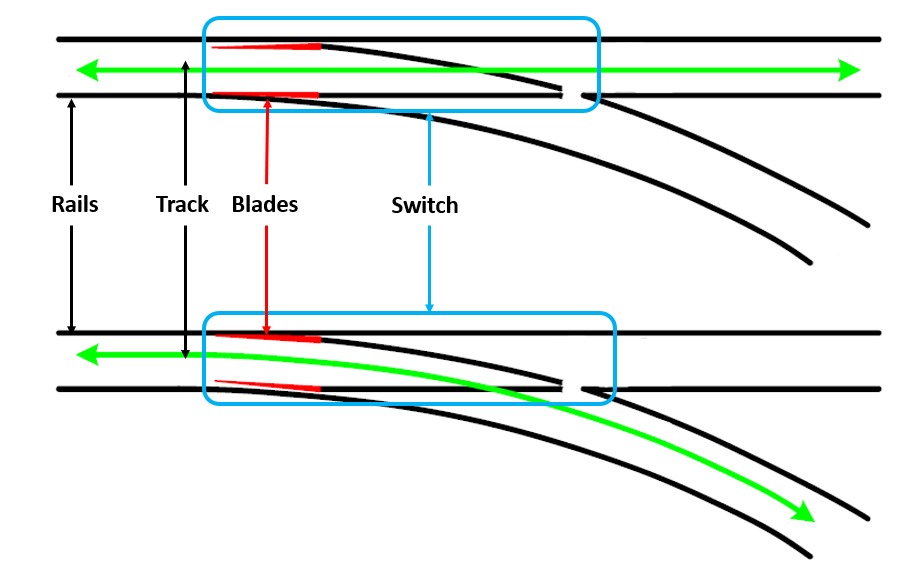
\includegraphics[scale=0.4]{figures/rail_anatomy.png}}
	\caption{Elements of the railway anatomy. Adapted from \cite{karakose2016detection}}
	\label{fig:railanatomy}
\end{figure}

The structure of the railroad is composed of two main elements: \textbf{rails}, long, metallic, parallel structures made to be in contact with the train and the \textbf{track gauge}, the area between the rails, on which wooden or concrete supports are placed in order to help maintain them. For simplicity and consistency with other works from the literature, we will refer to the latter element as the track. Rails used in the city by trams have the a similar structure. Another essential component of the railroad infrastructure is the switch. A switch is a simple, yet effective mechanism which allows the train to change its track through the movement of two rail extensions named blades. The blades have two states, one allows the train to continue its current course, while the other deviates it to another track. A schematic illustration of all the elements can be observed in Fig. \ref{fig:railanatomy}.

\begin{figure*}[htb]
    \centering
	\centerline{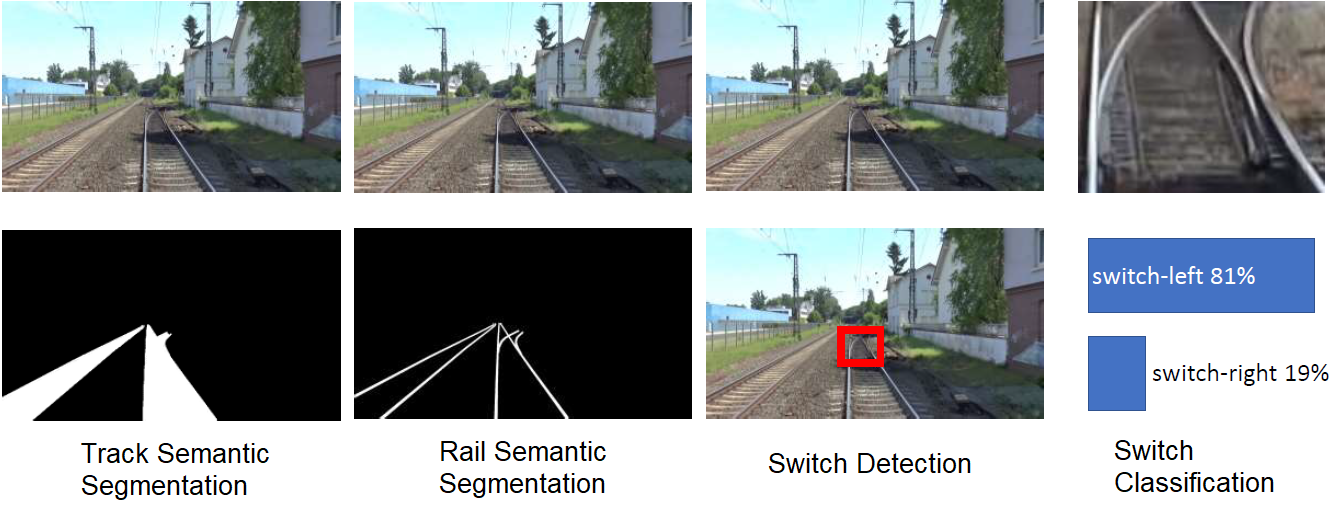
\includegraphics[scale=0.65]{figures/rail_tasks.png}}
	\caption{Example of tasks from the field of Railway Scene Understanding}
	\label{fig:railtasks}
\end{figure*}

Several main subfields of AI applications in railways are identified in works such as \cite{bevsinovic2021artificial} and \cite{tang2022literature}. One of these is Autonomous Driving and Control which studies 
intelligent techniques that would allow trains to travel with little or no human intervention. Automating 
such processes has the potential to increase fuel efficiency as each maneuver would be performed almost perfectly. In adjacent fields this is obtained through reinforcement learning. An essential step of future autonomous trains, which has to be tackled before, is scene understanding. In this compounded computer vision task, based on live video feed and, optionally, on other data from sensors such as lidars and radars, relevant information is extracted. This includes: the position and  topology of the railway track and the location and state of traffic lights, traffic signs and switches. Further information such as the presence of obstacles is also required in this type of safety-critical system. The totality of this information is necessary in any future autonomous trains as it informs the decision-making process.

Semantic segmentation, object detection and image classification are all required in order to obtain complete scene understanding in the Railway field. The topology of railroad can be extracted using either track semantic segmentation or rail semantic segmentation. In the former, each pixel from the original image is classified as either background or part of the rail-track. In the latter task,  the model has to distinguish between rails and everything else. This increases the difficulty as the thinness of the metallic structure requires finer, more precise segmentation.

Recognizing switches is another important task as understanding the state of this mechanism would allow an intelligent system to check whether or not it is bound to continue on the correct route and avoid accidents. This can be achieved by finding the location of the switch, than classifying the resulting crop. This process can be performed by two separate networks: one specialized in detection and the other responsible for classification of left and right switches. Alternatively, a single model can be trained in an end-to-end manner to perform both tasks simultaneously. An illustration of all previously described tasks can be seen in Fig \ref{fig:railtasks}.

Some works from the literature stand out due to their impact or impressive performance. First of all, most research in the field is conducted on the RailSem19 dataset \cite{zendel2019railsem19}, the most comprehensive set containing both object detection and semantic segmentation annotations. In track semantic segmentation, RailCNN \cite{belyaev2020railroad} is able to achieve a mean IoU of 93.1\%. A related, but more challenging task due to the required precision is rail segmentation. In \cite{alexandrescu2022dynamic}, the authors were able to obtain over 81\% IoU, although the final model is limited in terms of the inference speed.

 Unlike the segmentation task, switch detection and classification received little attention. Paper \cite{switch_classification} compares established backbones with a simple two-layer convolutional network for the task of switch classification, achieving up to 96\% accuracy. One of the only papers that approach switch detection is \cite{jahan2021deep}, in which a RetinaNet model \cite{lin2017focal} is employed on a private dataset achieving 95.9\% detection accuracy. In the same framework, the classification module of the detector obtained a 90.21\% accuracy. This being said, the same approach is able to obtain just a 8\% mean average precision on the RailSem19 dataset for the detection task.

The examination of these models reveals some limitations in their performance, indicating that there is room for improvement in addressing the identified constraints. Furthermore, it is noteworthy that a dedicated multi-task model tailored to address the nuances of this specific problem has yet to be developed. The absence of a customized solution underscores the ongoing need for advancements in the model architecture to effectively tackle the complexity of railway scene understanding.

We propose a novel multi-task architecture that combines a detection model and a segmentation one for learning to perform rail semantic segmentation, switch detection and switch classification simultaneously.
The model, named \textbf{UOLO}, also exploits traditional computer vision techniques and it is able to achieve state-of-the-art performance for the first two tasks, while respecting constraints which would make it applicable in real-time on an edge device. This work aims to provide answers to the following research questions. 

\begin{enumerate}
    \item[\textbf{RQ1}:] 
    How might multitask learning potentially enhance performance in rail scene understanding?
    \item[\textbf{RQ2}:] 
    What is the extent of the possible improvement obtained by leveraging classic computer vision approaches to enhance deep learning models?
\end{enumerate}

The structure of the rest of this paper is the following: Section \ref{relWork} describes related methods used for solving this task or a similar problem to it, Section \ref{sec:methodology} presents the proposed approach for the rails semantic segmentation task and Section \ref{results} describes the performed experiments  and presents the obtained results. Section \ref{conclusion} concludes the paper by offering an overview of the work and some future considerations.

\section{Related Work}
\label{relWork}

Switch identification is the task of detecting the location of switches placed on train tracks and classifying the direction in which they are oriented. The problem has been addressed till now from different perspectives: precise localisation of the rails was approached as a semantic segmentation task that focuses on classifying pixels into different categories (rails, tracks, backgrounds), while switch recognition was approached as a localisation and classification task solved as a detection problem.

\subsection{Railroad Semantic Segmentation}

In \cite{wang2019railnet}, the whole rail track is segmented. The authors propose a novel network for rail segmentation, RailNet which was trained and tested on a private dataset because at the time of its inception, RailSem19 was not published yet. The network which is able to perform inferences at a speed of 20 frames per second \textbf{(FPS)}, employs a ResNet50 as the backbone. The networks is divided into five stages. A decoder is developed in order to mirror the encoder stages and skip connections are added between the encoder and decoder in order to fuse high-level features with low-level features, starting from the second stage.

Before every upsampling, the feature map from the decoder is saved. This structure is inspired by the Feature Pyramid Networks \textbf{(FPN)}, architecture introduced in \cite{lin2017feature}. The resulting multi-scale information from the decoder is aggregated by first rescaling them to the same fixed dimension. This is achieved through a combination of the interpolation operation and the use of the region of interest pooling layer introduced in \cite{girshick2015fast}. One notable aspect of this method is the use of a novel loss function. The traditional cross entropy applied on the whole image is averaged with a loss which only takes into account the area surrounding the rail. The bounding box which perfectly encapsulates the segmented rail-track is computed and the same loss function is calculated only for this crop. In this way, the importance of the rail class is increased as most of the background is not taken into consideration for this computation. This is possible because the private dataset only contains images in which a single rail-track is present. This model outperforms Mask RCNN achieving almost 90\% IoU, exceeding the performance of the established network by around 3\%. This is especially impressive as the speed of the inference is also better.
%, as Mask RCNN runs at approximately 5 frames per second.

RailCNN, a model proposed in \cite{belyaev2020railroad}, is able to outperform this RailNet while preserving the real-time speed. The architecture is a U-Net model modified by replacing the skip connections with attention modules. Moreover, the encoder and decoder are connected with a spatial pyramid pooling (SPP) layer. A definitive characteristic of this method is the input size, as the models receives images with a high resolution of 2168 x 4096. This is a significant upgrade when compared to all other architectures proposed in the literature. The cost of this is only 3 FPS, the model being able to run at 17 frames per second. The increased image size allows for better segmentation of fine details, which would be otherwise impossible to extract from lower resolution images. Furthermore, the size of the input has a noteworthy practical use, as the model is able to segment rails found at further distances, reaching over 150 meters exceeding the previous maximum of  115 meters. This will be an important quality in future autonomous trains as having information earlier facilitates any decision making process. Another technique which improves the performance of this approach is online hard example mining \textbf{(OHEM)} \cite{shrivastava2016training}, allowing samples on which the model performs poorly to be sampled more often during training. RailCNN and RailNet are compared on different datasets, as the latter was trained on a private one. RailCNN is able to reach 93.1\% mean IoU for the rail track segmentation on RailSem19, improving the previous state-of-the-art by more than 4\%. 

For the, more challenging task of rail segmentation, a different architecture having the RailNet name has been proposed in \cite{li2020railnet}. This task is more difficult when compared to the previous one, as it requires a finer segmentation. What would have been a small mistake in the previous formulation of the task, has a noticeable negative impact as rails are extremely thin, especially when compared to the whole track. Moreover, the problem is far more unbalanced. Although challenging, segmenting rails instead of the whole rail-road has many benefits. First of all, thorough the combination of the rail segmentation with a post-processing algorithm we should be able to obtain the whole track, as the area between the parallel lines could be filled. Secondly, rail segmentation allows the inspection of this structure in task such as anomaly and defect prediction. Lastly, rail blades, which are part of the rail, indicate the position and state of switches.

To the best of our knowledge, RailNet \cite{li2020railnet} is the first approach which tackles the problem of rail segmentation. The proposed architecture combines a VGG16 backbone with a novel information aggregation module \textbf{(IAM)}. The purpose of this component is to fully exploit the spatial priors of rails including aspects like shape and spacing. The mechanism of an spatial convolutional-neural network \textbf{(SCNN)} is distilled in a single block which is able to learn strong local connections between rows and columns while also increasing the receptive field. The main idea behind the IAM is to compute a weight for all combinations of rows and columns. This is very similar to the attention mechanism, but heavily reduces the computational burden by restricting the weights to combinations of rows and columns. For this reason, the authors refer to this mechanism as "orthogonal attention". The model is trained on 5000 images and validated on 3500, using the focal loss \cite{lin2017focal} as a way to address the class imbalance. The introduction of this module is able to increase the mean IoU performance by 14\% reaching 54\%. From this point in the paper, all mentions of the RailNet model will refer to this architecture, unless stated otherwise.

Although it is not the focus of their work, paper \cite{jahan2021anomaly} investigates rail segmentation as a step in their anomaly detection pipelines. Two U-Net variants are employed. The authors conduct experiments with two encoders, namely VGG, as in the RailNet architecture, and ResNet. During their tests, the loss function choice is also investigated as experiments are made with weighted binary cross-entropy and focal losses with different 
$\alpha$ and $\gamma$
parameters. The best result 52.78\% mIoU on the RailSem19 dataset was obtained using the VGG encoder and focal loss with parameters alpha and gamma equal to 0.8 and 2, respectively. In \cite{alexandrescu2022dynamic}, the problem is tackled using the classic U-Net and ResUNet++ \cite{jha2019resunet_plus_plus} architectures, the weighted binary cross-entropy and the use of the dropout layer \cite{srivastava2014dropout}. When trained on 512x512 images U-Net outperforms its newer variants achieving 81\% mean IoU, while also exceeding the performance of RailNet. This being said, the network does not respect the constraint of being applicable in real-time applications. 

\subsection{Switch Detection and Classification}

Four main works from the literature were identified which approach either switch classification or the combined task of detection and classification. As mentioned previously, the authors of RailSem19 also attempt to provide initial baselines for their dataset, one of them being for switch classification. Using a DenseNet161 \cite{huang2017densely} crops of right switches and left switches are classified. The problem is extremely difficult as the only difference between the two comes in the form of the position of the blades, which are a small part of the rail. After some initial experiments, the authors decided to enlarge the crop from the initial bonding box context in order to capture more context, increasing the crop by 30\% on the x-axis and 125\% on the y-axis. The resulting 1460 left switches and 1539 right switches are augmented using multiple techniques such as perspective warps and rotations in order to increase the training set. After 20 epochs, the model reached 67\% accuracy showcasing the difficulty of this binary classification task.

In \cite{switch_classification}, the problem is extended from binary to a tertiary \ classification one, the third  class consisting of background crops. Four architectures are examined: VGG \cite{simonyan2014very}, ResNet \cite{he2016deep}, MobileNetV3 \cite{howard2019searching} and a two-layered convolutional network, named simple network \textbf{(SNet)}. Again, the initial context of the bounding box is extended. Experiments are conducted to find the best percentage of context enlargement. Moreover, the authors experiment with datasets in which switches with multiple enlargement factors are used. Images with less than 30 pixels were eliminated as the fine details required for this task were not distinguishable. Lastly, in some experiments the input is enriched with an extra channel containing the segmentation mask of the crop. The best results was obtained by the MobileNetV3 network, trained on multiple enlargement factors (1, 1.2, 1.35) having as input the normal RGB image. The network was pretrained on Image Net \cite{deng2009imagenet}. Although it removed some hard samples which would reduce the overall accuracy, this model achieved around 95\% accuracy for this difficult task. 


\begin{figure}[htb]
    \centering
	\centerline{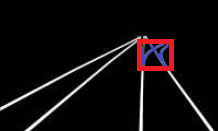
\includegraphics[scale=1.6]{figures/seminst.png}}
	\caption{Difference between rail semantic segmentation and instance segmentation when combined with switch detection. The white rail pixels are obtained only through semantic segmentation, as the detection task restrains the instance segmentation (blue) to the predicted bounding box.}
	\label{fig:semantic_vs_instance}
\end{figure}

\iffalse
\begin{figure*}[htb]
    \centering
	\centerline{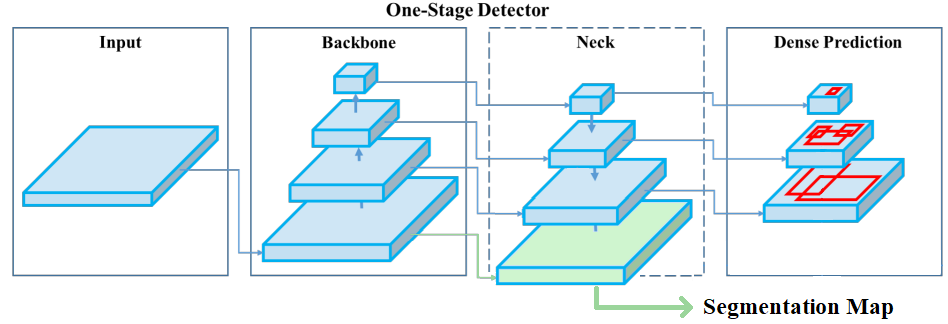
\includegraphics[scale=0.9]{figures/uolo2.png}}
	\caption{Overview of the proposed approach. Adapted from \cite{bochkovskiy2020yolov4}. The green feature map used to obtain the semantic segmentation prediction is exclusive to our proposed architecture.
        }
	\label{fig:uolo}
\end{figure*}
\fi

One of the first switch detection method employs classic computer vision techniques, in favour of deep learning. The algorithm proposed in \cite{karakose2016detection} is tested on a private dataset. When compared to the images from RailSem19, the ones used in this method are closer to the ground, resulting in a significantly increased quality of the rails. While this can increase accuracy, in practice it would not allow trains to detect or classify switches in time to react to the obtained information. Using the Canny edge detector \cite{canny1986computational} and Hough line transform \cite{duda1972use} intersection between rails which indicate the presence of switches are found. Using a series of computation which takes into account the positions, gradients and angles of the identified semantic lines left switches are identified correctly 82.7\% of times while the accuracy for the right-switch class reaches 88.4\%.

A deep learning approach based on the RetinaNet architecture for switch detection and classification is proposed in \cite{jahan2021deep}. The backbone of the network consists of a ResNet and a FPN. Taking as input images with a resolution of 960x540 the model is pretrained on the COCO dataset \cite{lin2014microsoft}. When trained on their own private dataset, this approach is able to reach 93.92\% validation mean average precision \textbf{(mAP)}. Unfortunately, due to inconsistencies in annotation, quality of images, various weather conditions and small sizes of objects the same method reaches only 8\% mAP on RailSem19. This real-time detector, which can run at 20 FPS, has a detection accuracy of 95.9\% and a classification accuracy of 90.21\%, when evaluated on the private dataset.

% Add information regarding our approach and what makes it unique

\section{Proposed Approach}
\label{sec:methodology}

To advance the current standards in comprehending railway scenes, we introduce an innovative multi-task framework named UOLO. This architecture merges the widely used YoloV5 object detector \cite{glenn_jocher_2020_4154370}, \cite{bochkovskiy2020yolov4} with the well-established UNet model \cite{ronneberger2015u} for semantic segmentation. Moreover, we augment this network by incorporating extra geometric features derived from conventional computer vision techniques.

\subsection{Preprocessing}

\begin{figure*}[htb]
    \centering
	\centerline{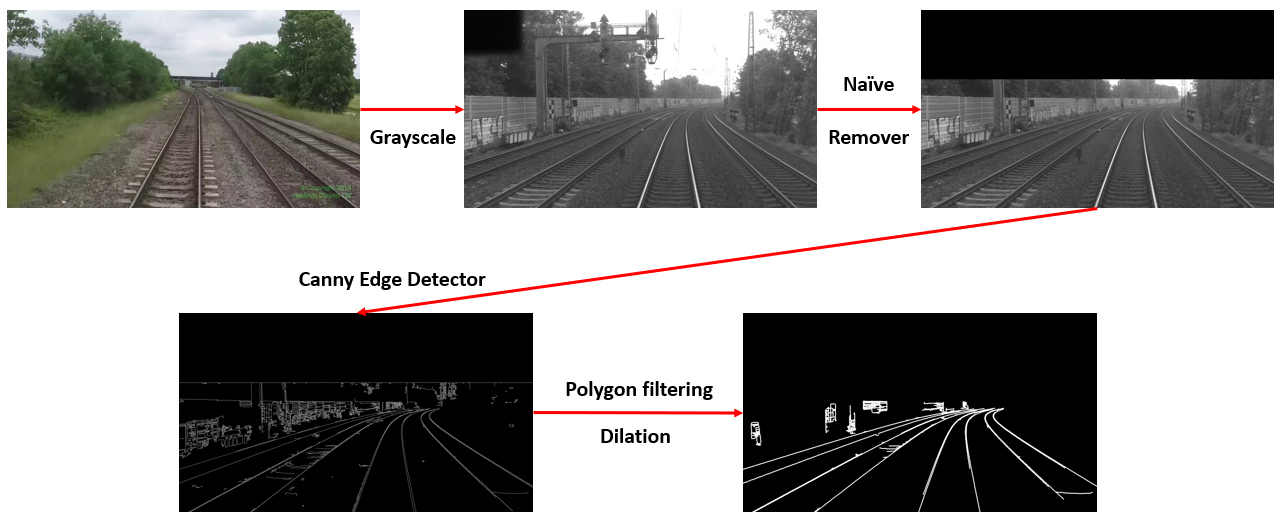
\includegraphics[scale=0.7]{figures/geometric_prior.png}}
	\caption{Steps of our classic computer vision preprocessing technique.}
	\label{fig:geometricprior}
\end{figure*}

An important step of our pipeline is the use of two preprocessing techniques. In the first one, bounding box enlargement is performed before training in order to facilitate the learning process. The second one generates an additional input channel, computed by using classic computer vision algorithms that are able to extract geometric information.

\subsubsection{Bounding Box Enlargement}
We facilitate the detection objective by preprocessing all bounding boxes from the dataset. This is an important step as YOLO-based architectures are known to be limited when it comes to smaller objects. We enlarge both the width and the height of each bounding box by altering their values through two distinct modalities: firstly, by directly augment them by an absolute (constant) value, and secondly, by the application of a relative (percentage-based) change:
\begin{equation}
\text{new\_width} = ( \text{width} + \alpha ) \cdot \beta
\end{equation}
\begin{equation}
\text{new\_height} = ( \text{height} + \alpha ) \cdot \beta
\end{equation}

%\textcolor{green}{si in YOLO si in YOLACT e la fel?  decoding-ul nu e pana la dimensiunea originala a imaginii?}

In the equations 1 and 2, $\alpha$ represents the absolute increase (in pixels) and $\beta$ the relative enlargement with $\alpha \in \{0, 50, 75, 100, 125, 150\}$ and $\beta \in \{90\%, 100\%, 110\%, 125\%, 150\%\}$.

All combinations are examined visually in order to grasp whether or not the preprocessed annotation occupies too much area in the image. To be noted that a absolute increase of 0 means that only the relative enlargement will be applied. We consider the absolute enlargement essential as it has a bigger effect on smaller bounding boxes, rather than on ones which already have a satisfactory dimension. The increase is done in a manner which preserves the center of the original annotation. For example, the absolute 50 pixel increase would result in the bounding box being extended with 25 pixels on all sizes. 
After the absolute increase is applied we continue with the relative enlargement. Some experiments were conducted with different increases for the height and width of the box, for we could not find a configuration worth pursuing so in the end the same increase was applied to both dimensions. Here, the value 1 is the neutral element as it keeps the bounding box as before the operation, leading to only the absolute transformation being applied. Another notable value is 0.9. The idea behind this was to attempt to bring the dimensions of bounding boxes closer together, by reducing larger box by a greater value. In practice, this preprocessing mostly yielded unpromising results. 
% \textcolor{green}{propoz urm e neclara; o poti reformula, te rog? 
% Larger values for both preprocessings for not considered as visually the resulting bounding boxes were more than large enough in some configurations.}
% } \textcolor{red}{Nu cred ca mai este nevoie de propozitia respectiva. Propun sa o stergem. (Voiam sa spun ca daca s-ar mari si mai mult BBoxurile nu ar fi in regula deoarece devin prea mari.}


%We propose the use of a constant enlargement, an increase based on a percentage of the initial size and a combination between the two. 
%All combinations are examined visually in order to grasp whether or not the preprocessed annotation occupies too much area in the image. For the constant enlargement we choose six possible values which will be used to increase both the width and the height of the original bounding box: 0, 50, 75, 100, 125, 150. To be noted that an increase of 0 means that only the percentage-based enlargement will be applied. We consider the constant enlargement essential as it has a bigger effect on smaller bounding boxes, rather than on ones which already have a satisfactory dimension. The increase is done in a manner which preserves the center of the original annotation. For example, the constant 50 pixel increase would result in the bounding box being extended with 25 pixels on all sizes. Five values are used for the percentage-based increase: 0.9, 1, 1.1, 1.25, 1.5. The original height and width are multiplied with this value. Some experiments were conducted with different increases for the height and width of the box, for we could not find a configuration worth pursuing so in the end the same increase was applied to both dimensions. Here, the value 1 is the neutral element as it keeps the bounding box as before the operation, leading to only the constant transformation being applied. Another notable value is 0.9. The idea behind this was to attempt to bring the dimensions of bounding boxes closer together, by reducing larger box by a greater value. In practice, this preprocessing yielded unpromising results. In all cases, the constant increase is applied before the percentage-based one. 
%\textcolor{green}{propoz urm e neclara; o poti reformula, te rog? 
%Larger values for both preprocessings for not considered as visually the resulting bounding boxes were more than large enough in some configurations.}


\subsubsection{Extra Geometric Input Channel}

Railways have a lot of embedded geometry inside their structure. The  rails are two parallel lines, which in many cases seem straight from the perspective of the ego-view camera. The presence of curves increase the overall complexity. Another fixed variable is the distance between the rails which is standardized. From the ego-view perspective as the rails are further away, closer to the horizon, they seem to get closer to each other or even intersect. All these aspects and more could be learned by the convolutional layers of our network, as these blocks can identify edges, shapes, textures and more. However, enhancing the model with additional geometric information, computed algorithmically, could facilitate the optimization process, reduce convergence time and even increase performance.

We propose a series of transformations, showcases in \textbf{Fig. \ref{fig:geometricprior}}, which have the purpose of offering a good prior for the rail extraction task. 
Given the input image before its fed through the model, a rail semantic segmentation mask is obtained by employing classic computer vision techniques. 
Due to known limitations of hand-crafted approaches, namely the difficulty of finding parameters that are general enough and perform well in multiple scenarios, the resulting segmentation mask would not have impressive results by itself. However, it offers a good starting point for the semantic segmentation task, while also offering extra information to the detection objective. The mask is concatenated to the original RGB image, resulting in an input that has 4 channels. 

The extra input channel or geometric prior is obtained by applying the following steps:
\begin{enumerate}
    \item RGB to Grayscale -  First, the RGB input image is transformed to grayscale, as features describing the colour are not required to identify rails.
    \item Naive Remover - We  eliminated the upper part of the images as we observed that rails are almost never present there due to the camera placement. 
    \item Edge Detection - Next, all edges are detected using Canny's algorithm \cite{canny1986computational}. 
    \item Polygon Approximation - Using the resulting contours, we can approximate polygons if the edges are close-enough to each other. This step is done via the Douglas-Peucker algorithm \cite{douglas1973algorithms} for polygon simplification. 
    \item Polygon Filtering - The resulting polygons are filtered based on their perimeter and number of sides. The polygons representing the rails should have a medium perimeter as defined by their long, but slim shape and a small number of sides as they are closely encapsulated by a rectangle shape. 
    \item Contour dilation - Lastly, because of the thinness of the result all remaining contours are dilated.
\end{enumerate}

For all the steps we employed the implementations from the open-source library, OpenCV \cite{opencv_library}. Hough line transform \cite{duda1972use} was also investigated, but the perspective of the camera often captures curves making the line not an effective simplification for the rails. Approaches that represent rails using this transformation, including \cite{karakose2016detection}, work due to the fact that the camera is closer to the ground, making the rails captured in the image seem more linear.

\subsection{Architectures}

We propose a novel architecture, starting from the established YoloV5 
\cite{bochkovskiy2020yolov4} \cite{glenn_jocher_2020_4154370}
object detection by adding a new path for the task of semantic segmentation. YoloV5 has been previously employed for multitask learning in which the detection objective is combined with instance segmentation 
\cite{bolya2019yolact}. 
In this scenario, 
the instance segmentation path is part of the already existing detection one, and the result obtained by the segmentation layers results in a finer-grained detection. Everything outside the detection bounding-box is ignored, which is not suitable for our complete railway scene understanding objective.

\begin{figure*}[htb]
    \centering
	\centerline{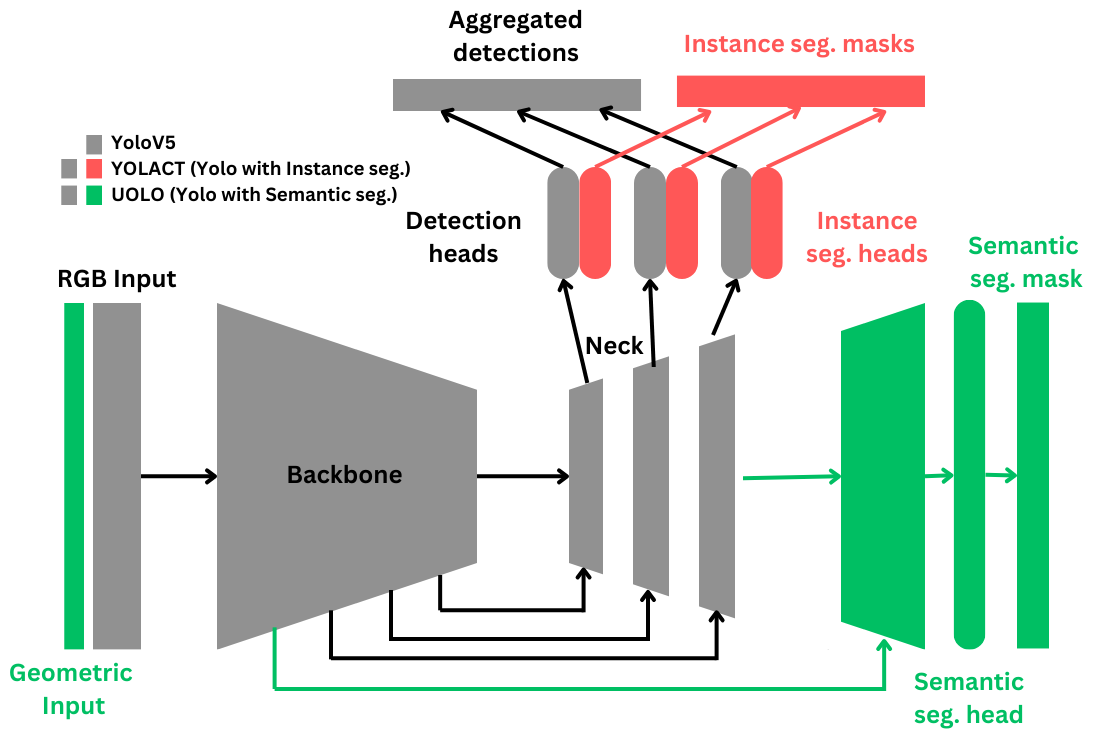
\includegraphics[scale=0.7]{figures/det_sem_instance3.png}}
	\caption{Comparison between YOLO \cite{bochkovskiy2020yolov4} \cite{glenn_jocher_2020_4154370}, YOLACT \cite{bolya2019yolact} and the proposed UOLO (Ours)}
	\label{fig:yoloactuolo}
\end{figure*}

% Desen instance vs semantic segmentation
As seen in Fig. \ref{fig:semantic_vs_instance}, tying the segmentation to the predicted detection bounding-box heavily limits the possible amount of information we can gather. In order to extract, all the rail pixels present in the image, through segmentation, while detection is also performed by the same network, the use of semantic segmentation is required, in the detriment of instance segmentation.

When attempting to detect switches, the location of railways is an important clue as switches are present only at the intersection of two railways. The orientation of the blades is the only element that allows the classification of switches, making rail segmentation an essential step in any autonomous train system. Using a segmentation model to detect rails, before the detection step is a viable approach, but it enforces stronger constraints on both models as the whole process is required to run in  real-time. For this reason, and as a way to also reduce memory requirements, the two models could be combined in a single one. Furthermore, we hypothesize that the two objectives are symbiotic leading to increased performance when the model learns them simultaneously. Multitask models also reduce computational costs during training, as they usually share a significant part of the individual architectures, allowing us to conduct more experiments or to train longer when compared to a traditional approach.

In our approach, the semantic segmentation path is added as a continuation of the decoding path of the detector's neck. The path consists of blocks made of convolutional and upsampling layers, enlarging the largest feature map from the decoding side until it reaches the original image resolutions. This additional path, consists of three decoding blocks. A block has two layers: a 3x3 convolution and an upsampling. The first layer is followed by an activation function, in the form of SiLU \cite{elfwing2018sigmoid}.

We combine low-level features from the backbone with high-level features from the neck through the use of skip connections. 
Shortcuts are added between the encoder backbone and the first two deconvolutional blocks from our semantic segmentation path, mirroring the use of skip-connections from the base Yolo architecture. A final 1x1 convolution, activated by the sigmoid function is employed in order to obtain the semantic segmentation prediction.

The resulting segmentation architecture resembles the U-Net model \cite{ronneberger2015u}. First of all, the structures of the networks are virtually the same, both models having a encoding path, a decoding path and skip-connections between the corresponding feature maps from the two. However, the structure of these elements differs as we build the proposed approach upon the YoloV5 architecture. Since the proposal of U-Net, the relatively simple encoder has been replaced by more complex feature extractors, In Yolo, and in our proposed model, a Cross Stage Partial Network (\textbf{CSPNetwork}) \cite{wang2020cspnet} is used as the backbone, to reduce computational cost while maintaining the performance.

Another difference between the classic U-Net, and the proposed model is the use of the Spatial Pyramid Pooling (\textbf{SPP}) \cite{hezhang2015spp}. This pooling approach was found to be beneficial is multiple computer vision tasks including object detection and semantic segmentation as it combined features from multiple scales.

The proposed multitask approach has  two heads, one for each task. The detection head of most Yolo architectures is used, in which three loss functions are computed: box loss, object loss and classification loss. The first one is responsible for teaching the model the position and dimension of objects with the help of anchors. It is computed as the IoU between the predicted boxes and a real ones. The second one comes in the form of objectness or the probability of having an object in a predicted box. This can be seen as a classification between background and objects of interests, where the ground-truth is given by the IoU computed for the previous loss.

If the detector is also tasked with classing the objects into multiple classes, as in our case, a softmax layer is also added to the detection head and cross-entropy loss is applied to the pipeline. The additional segmentation tasks adds a forth loss to the process, computed in the segmentation head. As the problem requires only two-classes, we employ binary cross-entropy.

We name the resulting network \textit{U Only Look Once} or \textbf{UOLO}, for short. An overview illustrating this approach can be observed in \textbf{Fig. \ref{fig:yoloactuolo}}.

When compared to already existing hybrids which combine detection and instance segmentation, including YOLACT, UOLO covers an important niche. Instance segmentation can be seen as a finer form of detection thus existing architectures enhance the detection heads allowing them to perform instance segmentation. This symbiosis between the detection and instance segmentation tasks leads to impressive results but yields the instance segmentation head blind outside of predicted bounding boxes. In UOLO, outside of sharing extracted features from the encoder, the detection and segmentation heads are untangled, allowing the model to segment the image even if no object is found during the detection step.

\iffalse
\textcolor{red}{as evidentia avantajele teoretice ale abordarii propuse (iar in sectiunea de discutii le-as relua prezentarea, legandu-le de rezultatele numerice obtinute):
1. timpul redus pt training si/sau inferenta prin folosirea unui model multi-task
2. model tailored pt switch recognition/identification
3. altele daca mai sunt la nivel teoretic}
\fi

As a multitask model, UOLO has numerous advantages. Firstly, training and inference time are lower when compared to the prospect of having two individual networks, one for each task. Moreover, the multitask objective can lead to improved performance in both tasks as the encoder is compelled to learned general features applicable for two problems. The preprocessing steps tailor the approach for switch recognition and rail semantic segmentation, preprocessing which can be performed in real-time due to the high inference speed of the UOLO networks.


\section{Results}
\label{results}

\subsection{Dataset}

RailSem19 \cite{zendel2019railsem19} is the most comprehensive dataset for ego-view perspective scene understanding for trains and trams. Consisting of 8500 annotated images extracted from public videos filmed from locomotives and trams, the dataset has an annotation for object detection and semantic segmentation. The former were manually annotated using various shapes like bounding-boxes for switches and splines for rails. The semantic labels were annotated using a semi-supervised approach based on the existing manual annotations, resulting in some inconsistencies in the dataset. The worst case of these limitations comes in the form of a few images in which the rail annotations are completely missing. 

The dataset offers multiple types of hand-labeled geometric annotations including splines for rails, polygons for persons, cars or fences and bounding-boxes for left, right and unknown switches. In total over 110000 annotations which are part of 21 classes are present in this dataset. Out of these 21, seven of them have the potential to occlude the rail track. For our use case, we can exploit the presence of three classes: switch-left, switch-right, and unknown-switch having 1965, 2083, and 2491 instances. 

In terms of semantic labels, 20 classes are annotated in the dataset. When compared to previous semantic segmentations which have some rail annotations like CityScapes \cite{cordts2016cityscapes}
, RailSem19 has three main advantages. Firstly, all images are from the ego-view perspective, which is a realistic position of a camera in future autonomous trains. Secondly, the rails and track are annotated with different labels, allowing more flexibility in the training process, resulting in better scene understanding. Lastly, five new rail specific classes were introduced including annotation for tram tracks and rail-embedded, the latter referring to the tram rail which is integrated in existing roads. In most of our experiments we are only concerned with the rail and rail-embedded classes. To compare with other state-of-the-art approaches we also perform track segmentation in which we also segment the rail-track and tram-tracks. We consider the rails for trains and trams similar enough in order to use both sets of images in our experiments. 

\subsection{Prerequisites}

During our experiments we test our model using different configuration of the RailSem19 dataset. Depending on the aim of the test we decided whether or not to use unknown switches or images with no switches. The number of images containing a certain type of switch and the total number of instances from that class are presented in Table \ref{tab:dataDistribution}. 

\begin{table}[h]
        \centering
        \caption{Data distribution}
        \begin{tabular}{c|c|c}
             Type           & \# images & \# instances \\ \hline
             left switch    & 1447         & 1963 \\ \hline
             right switch   & 1963         & 2080 \\ \hline
             unknown switch & 1515         & 2490 \\ \hline
             no switch      & 5736         & - \\ \hline
        \end{tabular}                        
        \label{tab:dataDistribution}
    \end{table}

The following scenarios are considered:
\begin{itemize}
    \item $Scenario_1$ = left switch + right switch + unknown switch + no switch
    \item $Scenario_2$ = left switch + right switch + no switch
    \item $Scenario_3$ = left switch + right switch + unknown switch
    \item $Scenario_4$ = left switch + right switch 
    \item $Scenario_5$ = left switch + right switch + bounding box preprocessing
    \item $Scenario_6$ = left switch + right switch + bounding box preprocessing + geometric preprocessing
    
\end{itemize}

We evaluate our multi-task model using four main metrics. For the detection task we compute the mean-average precision (mAP) at an intersection-over-union (IoU) threshold of 50\%, meaning that all predicted boxes which have an IoU of less than 50\% will be considered false positives. We refer to this metric as mAP@50 full. In order to separate the performance of the detection and classification components of our network we compute the same metric without taking into account the predicted class thus evaluating only the detection. We refer to the resulting metric as mAP@50 det. 

For the segmentation task we compute the rail IoU and the backgroud IoU. Because the performance for the latter is not our main focus we report the rail IoU and the mean IoU (mIoU) which averages the two.

\subsection{Experiments}

In this section we will present the numerical results of our experiments performed on the scenarios described above.

\subsubsection{Switch identification in raw images}

The complete list of performance values obtained using YoloV5, which will be used as a baseline are presented in \textbf{Table \ref{tab:exp_yolov5_railsem19_subsets2}}. This experiment is conducted in order to measure the performance
of the detector head
in different scenarios 
% \textcolor{green}{it is not meant to be used to draw any conclusion regarding the best choice of images, as the subsets result in instances of the same task with different difficulties.}
% %eu am inteles de ce ai facut acest experiment, dar as evita afirmatii de genul: "it is not meant to be used to draw any conclusion"; eu as zice ca scopul acestui experiment e sa fixeze un bound / o limita / o referinta, utila in experimentele urmatoare}
and offer us a baseline value for the performance, which can be further used in the following experiments.

We do not perform classification, thus we do not obtain a  mAP@50 full score on the first two scenarios as the presence of unknown switches makes the task cumbersome. The model is unable to learn to concept of an "unknown switch", which is an unclear left or right switch, from human perspective, without a class label.

\iffalse
\begin{table}[ht]
    \centering
    \caption{YoloV5 detection performance on RailSem19 subsets.
    }
    \begin{tabular}{cccc}
    \hline
   \begin{tabular}{@{}c@{}}\textbf{Unknown switches} \\ \textbf{No switches} \end{tabular} & \textbf{No. images} & \textbf{mAP@50 det} & \textbf{mAP@50 full} \\
     \hline\hline
     \begin{tabular}{@{}c@{}}Yes\\ Yes\end{tabular} $Scenario_1$ & 8500 & 35.2\% & - \\ 
     \hline
     \begin{tabular}{@{}c@{}}Yes\\ No\end{tabular} $Scenario_2$ & 6976 & 37.6\% & - \\ 
     \hline
     \begin{tabular}{@{}c@{}}No\\ Yes\end{tabular} $Scenario_3$ & 2764 & 30.9\% & 17.0\% \\ 
     \hline
     \begin{tabular}{@{}c@{}} No\\ No\end{tabular} $Scenario_4$& 1240 & \textbf{43.0\%} & \textbf{23.6\%} \\
     \hline
    \end{tabular}
    \label{tab:exp_yolov5_railsem19_subsets}
\end{table}
\fi


\begin{table*}[ht]
    \centering
    \caption{YoloV5 and UOLO detection and segmentation performance on RailSem19 subsets.}
    \begin{tabular}{cccccccc}
    \hline 
    \multirow{2}{*}{\textbf{Scenario}} & \multirow{2}{*}{\textbf{No. images}} & \multicolumn{2}{c}{\textbf{mAP@50 det}} & \multicolumn{2}{c}{\textbf{mAP@50 full}} & \textbf{meanIoU} & \textbf{railIoU} \\
    \cline{3-8} & & YoloV5 & UOLO & YoloV5 & UOLO & UOLO & UOLO \\
     \hline\hline
     $Scenario_1$ & 8500 & 35.2\% & 35.6\% & - & - & 61.3\% & 26.5\%\\ 
     \hline
     $Scenario_2$ & 6976 & 37.6\% & \textbf{44.0\%} & - & - & 69.6\% & 42.0\%\\ 
     \hline
     $Scenario_3$ & 2764 & 30.9\% & 29.6\% & 17.0\% & 17.0\% & 55.1\% & 14.5\%\\ 
     \hline
     $Scenario_4$& 1240 & 43.0\% & 43.8\% & 23.6\% & 23.8\% & 68.3\% & 39.3\%\\
     \hline
     $Scenario_5$ & 1240 & - & 86.2\% & - & 51.3\% & 69.3\% & 41.2\% \\
     \hline
     $Scenario_6$ & 1240 & - & \textbf{87.0\%} & - & 51.4\% & \textbf{81.2\%} & \textbf{64.1\%} \\
     \hline
    \end{tabular}
    \label{tab:exp_yolov5_railsem19_subsets2}
\end{table*}

To quantify the capabilities of the proposed UOLO, we run the same experiments using this architecture. In almost all scenarios, we can observe that the use of the multi-task objective leads to better performance for the detection. The most notable example of this is for the subset with unknown switches and no images that do not contain switches  
(Scenario 3).
In that case, the performance is increased from 37.6\% to 44.0\%. The complete list of results is presented in \textbf{Table \ref{tab:exp_yolov5_railsem19_subsets2}}.

\iffalse
\begin{table}[ht]
    \centering
    \caption{Comparison between YoloV5 and Uolo detection performance on RailSem19 subsets.}
    \begin{tabular}{ccc}
    \hline
   \begin{tabular}{@{}c@{}}\textbf{Unknown switches} \\ \textbf{No switches} \end{tabular}  & \begin{tabular}{@{}c@{}}\textbf{YoloV5}\\ \textbf{mAP det $\setminus$ full}\end{tabular} & \begin{tabular}{@{}c@{}}\textbf{Uolo}\\ \textbf{mAP det $\setminus$ full}\end{tabular} \\
     \hline\hline
     \begin{tabular}{@{}c@{}}Yes\\ Yes\end{tabular} $Scenario_1$& 35.2\% & 35.6\% \\  
     \hline
     \begin{tabular}{@{}c@{}}Yes\\ No\end{tabular}  $Scenario_2$& 37.6\% & \textbf{44.0\%} \\ 
     \hline
     \begin{tabular}{@{}c@{}}No\\ Yes\end{tabular}  $Scenario_3$& \begin{tabular}{@{}c@{}}30.9\% \\ 17.0\%\end{tabular} &  \begin{tabular}{@{}c@{}}29.6\% \\ 17.0\%\end{tabular}\\  
     \hline
     \begin{tabular}{@{}c@{}} No\\ No\end{tabular} $Scenario_4$& \begin{tabular}{@{}c@{}}43.0\% \\ 23.6\%\end{tabular} & \begin{tabular}{@{}c@{}}43.8\% \\ \textbf{23.8\%}\end{tabular} \\
     \hline
    \end{tabular}
    \label{tab:exp_uolo_railsem19_subsets3}
\end{table}
\fi

\subsubsection{Rail segmentation in raw images}

Besides slightly outperforming the single-task YOLO architecture in the detection problem, UOLO performs rail semantic segmentation at the same time. The results obtained in the same initial four scenarios can be observed in \textbf{Table \ref{tab:exp_uolo_seg_railsem19_subsets}}. In the detection objective, it was expected to have worse performance when images containing no switches were used as it 
they created an imbalance between true-positives and true-negatives. In semantic segmentation of the rails, we expect that the extra 5706 images containing no switch, but having rail semantic labels would improve the performance of this objective. However, the best performance is achieved when the images with no switches are eliminated 
from the training set. 
Further investigation shows that the limitations of the semi-supervised semantic annotation process are most prevalent in those images. As the automatic part of the labeling process is conducted based on guidance inferred from the object detection annotations, the images with no switches have semantic labels of worse quality. The most extreme scenario in which the dataset has to suffer is when the rail annotation is completely missing. Using images in which at least one switch is present helps us address this issue to a certain extent, explaining the drastic increase in performance.

\begin{table}[ht]
    \centering
    \caption{UOLO performance on RailSem19 subsets.
    % \textcolor{green}{\\sunt rezultate obtinute cu YoloV5 sau cu UOLO? in text se spune ca sunt obtinute cu UOLO.\textcolor{red}{Cu UOLO.}}
    }
    \begin{tabular}{cccc}
    \hline
   \begin{tabular}{@{}c@{}}\textbf{Unknown switches} \\ \textbf{No switches} \end{tabular} & \textbf{No. images} & \textbf{mean IoU} & \textbf{rail IoU} \\
     \hline\hline
     \begin{tabular}{@{}c@{}}Yes\\ Yes\end{tabular} $Scenario_1$& 8500 & 61.3\% & 26.5\% \\ 
     \hline
     \begin{tabular}{@{}c@{}}Yes\\ No\end{tabular} $Scenario_2$& 6976 & 69.6\% & 42\% \\
     \hline
     \begin{tabular}{@{}c@{}}No\\ Yes\end{tabular} $Scenario_3$& 2764 & 55.1\% & 14.5\% \\ 
     \hline
     \begin{tabular}{@{}c@{}} No\\ No\end{tabular} $Scenario_4$& 1240 & 68.3\% & 39.3\% \\
     \hline
    \end{tabular}
    \label{tab:exp_uolo_seg_railsem19_subsets}
\end{table}

\subsubsection{Switch identification and rail segmentation in preprocessed images}

After these initial experiments which showcased the potential of multi-task learning, we focus our attention on preprocessing the input images. We enlarge the initial annotation in order to capture further information which should facilitate the switch detection performance. The positive impact should be even greater for the switch classification task, in which the supplementary context is absolutely necessary, as without the blades there is no distinguishable characteristic in switches.

\begin{figure*}[htb]
    \centering
	\centerline{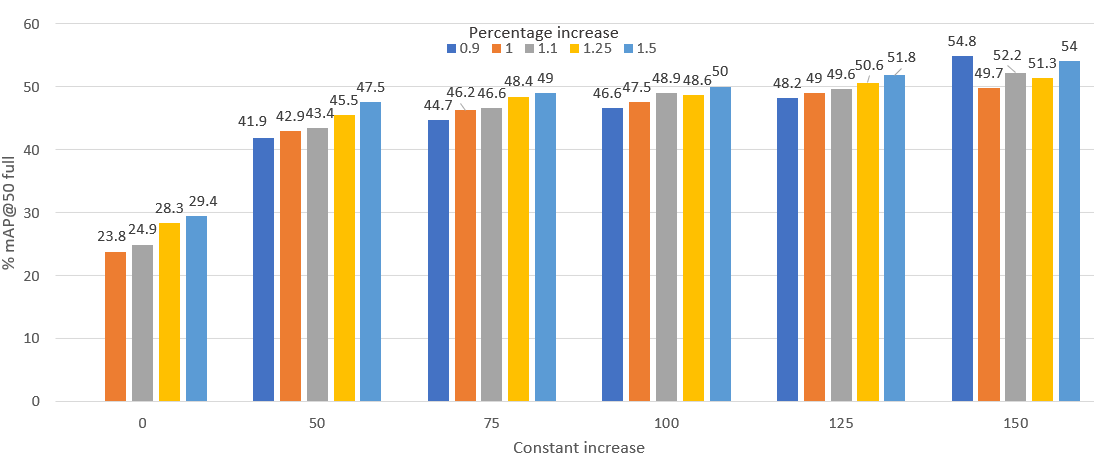
\includegraphics[scale=0.6]{figures/switch_preprocessing2.png}}
	\caption{Comparison between combinations of absolute and relative switch enlargement based on mAP@50 full.}
    % \textcolor{green}{oare daca ai pune pe axa Ox cresterile cantitative si cu culori sa diferentiezi modificarile procentuale nu s-ar alinia mai bine cu explicatia din text?\\ \textcolor{red}{Ar fi mai bine asa, voi reface graficul (Refacut).}
    % In plus, in tabele valorile pt mAP sunt date pe scara (0,1), aici, in figura, sunt pe scara (0, 100); ar fi bine sa se foloseasca aceeasi scara \textcolor{red}{Nu incapeau in grafic in varianta (0,1). Voi mofica sa fie uniform.}
	\label{fig:switch_enlargement_exp}
\end{figure*}



In \textbf{Fig. \ref{fig:switch_enlargement_exp}}, a comparison between the enlargement values can be observed, based on the mAP@50 performance on both the detection and classification 
for \textit{Scenario}$_5$. 
In most cases, as the enlargement increases the performance is also improved. The only combinations of fixed and relative increase we do not experiment with is the one with no absolute increase in which the dimensions would be multiplied by 0.9. We made the choice to omit this combinations as it defeats the purpose of enlarging bounding boxes. The remaining results obtained by combining this relative reduction with absolute increases suggest it has no beneficial effect until a larger fixed increase like 150 is used. For that pair, the best mAP@50 full value is obtained, specifically 54.8\%. 

As the extra input channels offers a first segmentation mask which requires refinement, the most noticeable impact
is seen in the mean IoU obtained by the segmentation path, whose performance is increased by more than 10\% IoU, as observed in \textbf{Table \ref{tab:geometric_preprocess}}. When it comes to the rail IoU the previous value, 41.2\% drastically rises to 60.6\%.  The performance of detection and classification is also slightly increased.

The proposed UOLO is competitive in rail semantic segmentation as seen in Table \ref{table:rail_sota_approaches}, a task in which we outperform the best-reported performance by 0.2\%, while respecting real-time constraints. In switch detection, we are able to obtain up to 87\% mAP an impressive value for the RailSem19 dataset, on which due to limitations in annotation no other notable model was proposed. On other private datasets, RetinaNet \cite{jahan2021deep} reaches over 95\%, but we are unable to test our approach on this data. These results are showcased in Table \ref{table:switch_det_approaches}.

\begin{table}[ht]
    \centering
    \caption{Impact of the geometric preprocessing. Model trained on images containing only left and right switches
    % \textcolor{green}{1. nu ar merita adaugata mean IoU pt switches?\\ 
    % \textcolor{red}{Intr-un fel mean IoU-ul pt switches e parte din mAP, dar se poate adauga ca sa fie completa analiza}
    % 2. tb reamintit scenariul in care esti, corespunzator imaginilor folosite (left + right?)}
    }
    \begin{tabular}{ccccc}
    \hline
   \begin{tabular}{@{}c@{}}\textbf{Geometric} \\ \textbf{Preprocess} \end{tabular} & \textbf{mean IoU} & \textbf{rail IoU} & \textbf{mAP det} & \textbf{mAP full} \\
     \hline\hline
      No $Scenario_5$ & 69.3\% & 41.2\% & 86.2\% & 51.3\% \\ 
     \hline
     Yes $Scenario_6$ & 81.2\% & 64.1 \% & 87.0\% & 51.4\% \\
     \hline
    \end{tabular}
    \label{tab:geometric_preprocess}
\end{table}

\subsubsection{Rail-track segmentation in preprocessed images}

%We also run an experiment in which we substitute the \sout{guard-}rail semantic segmentation task for rail-track semantic segmentation. In this task, applied to the images from the $Scenario_6$, we achieve a mean IoU of 93.5\%, exceeding the previous best performance from the literature achieved by RailCNN \cite{belyaev2020railroad} on smaller images while also performing detection. The performance of the switch detector does not differ from the one obtained when the objective is combined with \sout{guard-}rail semantic segmentation.

We run an additional experiment in which we tackle a different but related segmentation problem. With the same architecture and parameters we attempt to segment the whole railroad, including both rails and the track. Starting from Scenario 6 we add the track pixels to the ground-truth segmentation mask, with the same label as the rail pixels. We will refer to this task as rail track semantic segmentation in order to be consistent with the literature.

The resulting multitask approach which combines switch detection and the new rail track binary segmentation tasks allows us to compare the performance of UOLO with existing approaches from the literature. We were able to reach a mean IoU of 93.5\% exceeding the most performant existing approach, RailCNN \cite{belyaev2020railroad} by 0.4\%, as seen in Table \ref{table:track_approaches}. 

% add tables for comparison with SOTA
\begin{table}[h!]
\begin{center}
\caption{Rail semantic segmentation method comparison.
}
\begin{tabular}{c c c c} 
 \hline
 \textbf{Method} & \textbf{mean IoU} & \textbf{rail IoU} & \textbf{FPS}\\ [0.5ex] 
 \hline\hline
 RailNet \cite{li2020railnet} & 54.0\% & - & 5 \\ 
 VGG U-Net \cite{jahan2021anomaly} & 52.7\% & - & \textbf{27}\\
 U-Net \cite{alexandrescu2022dynamic} & 81.0\% & 63.0\% & 4 \\ 
 \hline
 UOLO & \textbf{81.2\%} & \textbf{64.1\%} & 22 \\ [1ex] 
 \hline
\end{tabular}
\label{table:rail_sota_approaches}
\end{center}
\end{table}

Despite all these encouraging results, the limitation of this proposed multitask approach is the switch classification which does not exceed 66\%. This weakness suggests, that at least at the moment the switch classification task may require a specialized network.

%\textcolor{blue}{
%Although the main focus of this work was to combine switch detection with rail segmentation, we also conduct an experiment in which we attempt to segment the whole rail-track. Using the same configuration described for the rail semantic segmentation we are able to outperform existing approaches by reaching an mIoU of 93.5\% as seen in Table \ref{table:track_approaches}.
%}

%Lastly, the limitation of this 
%\textcolor{red}{proposed} 
%multitask approach is the switch classification which does not exceed 66\%. This weakness suggests, that at least at the moment the task requires a specialized network.


\begin{table}[h!]
\begin{center}
\caption{Switch Detection method comparison.
}
\begin{tabular}{c c c c} 
 \hline
 \textbf{Method} & \textbf{Dataset} & \textbf{\begin{tabular}{@{}c@{}}mAP@50 + \\ full\end{tabular}} & \textbf{FPS}\\ [0.5ex] 
 \hline\hline
  \begin{tabular}{@{}c@{}}Canny + \\ Hough Line Transform\end{tabular}
  \cite{karakose2016detection} & Private & 85.5\%  & - \\
 RetinaNet \cite{jahan2021deep} & Private & \textbf{95.9\%}  & 
 \textbf{25} \\ 
 RetinaNet \cite{jahan2021deep} & RailSem19 & 8.0\% & 25\\
 \hline
 UOLO & \begin{tabular}{@{}c@{}}Preprocessed\\ RailSem19\end{tabular}  & \textbf{87.3\%} & 22 \\ [1ex] 
 \hline
\end{tabular}
\label{table:switch_det_approaches}
\end{center}
\end{table}

\subsection{Disscussion}

Through these experiments, we obtained informed answers to our research questions. First of all, multi-task learning improves the performance of both objectives, while being more computationally expensive than the two individual networks by themselves. Secondly, traditional computer vision can lead to notable improvements, at least in the railway scene understanding field where the existing geometry of the rails allows hand-crafted features obtained through classic algorithms to enhance the performance in both detection and rail semantic segmentation.

\begin{table}[h!]
\begin{center}
\caption{Rail track semantic segmentation method comparison.}
\begin{tabular}{c c c c} 
 \hline
 \textbf{Method} & \textbf{mean IoU} & \textbf{rail-track IoU} & \textbf{FPS}\\ [0.5ex] 
 \hline\hline
 U-Net \cite{katar2022automated} & 89.1\% & - & - \\ 
 RailNet \cite{wang2019railnet} & 89.8\% & - & 20 \\ 
 RailCNN \cite{belyaev2020railroad} & 93.1\% & - & 17\\
 \hline
 UOLO & \textbf{93.5\%} & \textbf{88.4\%} & \textbf{22} \\ [1ex] 
 \hline
\end{tabular}
\label{table:track_approaches}
\end{center}
\end{table}

While analysing the results and conclusions for our research question we have to take into account that all experiments were conducted on a single dataset. This threat is hard to overcome as, to the best of our knowledge, there are no other public datasets specialized in ego-view railway vision. 

A multi-task model exhibits temporal and memory efficiency across both the training and testing phases. In the training phase, the model's capacity to concurrently address multiple tasks speeds up the learning process, while in the testing phase the model demonstrates efficiency in processing input images and correctly classify the identified switches. 


\iffalse
\begin{comment}
\subsection{Experiments}

Before committing ourselves to the YoloV5 architecture, we experimented with numerous established detectors. RetinaNet, R-CNN, YoloV4, YoloV7 and even YoloV8 are just some of the models considered for the switch detection task. All experiments were conducted on the \textcolor{red}{original} 
\textcolor{green}{original or raw (instead of "normal")}
dataset without applying any preprocessing. The results were far from encouraging, the best performance being achieved by YoloV5, the network reaching only 0.352 mAP@50 for the detection without taking into consideration the classification.

First of all we analyse four subsets of the raw RailSem19. These subsets are built based on two variable: the presence of images with no switches and the presence of images in which at least one unknown switch is present. We report the mAP@50 for the detection class (\textit{mAP@50 det}), in which all switches are considered as being part of the same category. In the scenarios in which the unknown switch is not present we are also able to perform switch classification as part of the detection process. This result is given under the \textit{mAP@50 full} column, when it is applicable. The complete list of performance values obtained using YoloV5, which will be used as a baseline are presented in \textbf{Table \ref{tab:exp_yolov5_railsem19_subsets}}. This experiment is conducted in order to measure the performance in different scenarios, \textcolor{green}{it is not meant to be used to draw any conclusion regarding the best choice of images, as the subsets result in instances of the same task with different difficulties.\\
eu am inteles de ce ai facut acest experiment, dar as evita afirmatii de genul: "it is not meant to be used to draw any conclusion"; eu as zice ca scopul acestui experiment e sa fixeze un bound / o limita / o referinta, utila in experimentele urmatoare}
\textcolor{red}{and offer us a baseline value for the performance, which can be further used in the following experiments.}

\begin{table}[ht]
    \centering
    \caption{YoloV5 performance on RailSem19 subsets.}
    \begin{tabular}{cccc}
    \hline
   \begin{tabular}{@{}c@{}}\textbf{Unknown switches} \\ \textbf{No switches} \end{tabular} & \textbf{No. images} & \textbf{mAP@50 det} & \textbf{mAP@50 full} \\
     \hline\hline
     \begin{tabular}{@{}c@{}}Yes\\ Yes\end{tabular} & 8500 & 0.352 & - \\ 
     \hline
     \begin{tabular}{@{}c@{}}Yes\\ No\end{tabular} & 6976 & 0.376 & - \\ 
     \hline
     \begin{tabular}{@{}c@{}}No\\ Yes\end{tabular} & 2764 & 0.309 & 0.170 \\ 
     \hline
     \begin{tabular}{@{}c@{}} No\\ No\end{tabular} & 1240 & \textbf{0.430} & \textbf{0.236} \\
     \hline
    \end{tabular}
    \label{tab:exp_yolov5_railsem19_subsets}
\end{table}

To quantify the capabilities of the proposed UOLO, we run the same experiments using this architecture. In almost all scenarios, we can observe that the use of the multi-task objective leads to better performance for the detection. The most notable example of this is for the subset with unknown switches and no images which do not contain switches. In that case, the performance is increased from 0.376 to 0.440. The complete list of results is presented in \textbf{Table \ref{tab:exp_uolo_railsem19_subsets}}.

\begin{table}[ht]
    \centering
    \caption{Comparison between YoloV5 and Uolo detection performance on RailSem19 subsets.}
    \begin{tabular}{ccc}
    \hline
   \begin{tabular}{@{}c@{}}\textbf{Unknown switches} \\ \textbf{No switches} \end{tabular}  & \begin{tabular}{@{}c@{}}\textbf{YoloV5}\\ \textbf{mAP det $\setminus$ full}\end{tabular} & \begin{tabular}{@{}c@{}}\textbf{Uolo}\\ \textbf{mAP det $\setminus$ full}\end{tabular} \\
     \hline\hline
     \begin{tabular}{@{}c@{}}Yes\\ Yes\end{tabular}  & 0.352 & 0.356 \\  
     \hline
     \begin{tabular}{@{}c@{}}Yes\\ No\end{tabular}  & 0.376 & \textbf{0.440} \\ 
     \hline
     \begin{tabular}{@{}c@{}}No\\ Yes\end{tabular}  & \begin{tabular}{@{}c@{}}0.309 \\ 0.170\end{tabular} &  \begin{tabular}{@{}c@{}}0.296 \\ 0.170\end{tabular}\\  
     \hline
     \begin{tabular}{@{}c@{}} No\\ No\end{tabular} & \begin{tabular}{@{}c@{}}0.430 \\ 0.236\end{tabular} & \begin{tabular}{@{}c@{}}0.438 \\ \textbf{0.238}\end{tabular} \\
     \hline
    \end{tabular}
    \label{tab:exp_uolo_railsem19_subsets}
\end{table}


\begin{figure*}[htb]
    \centering
	\centerline{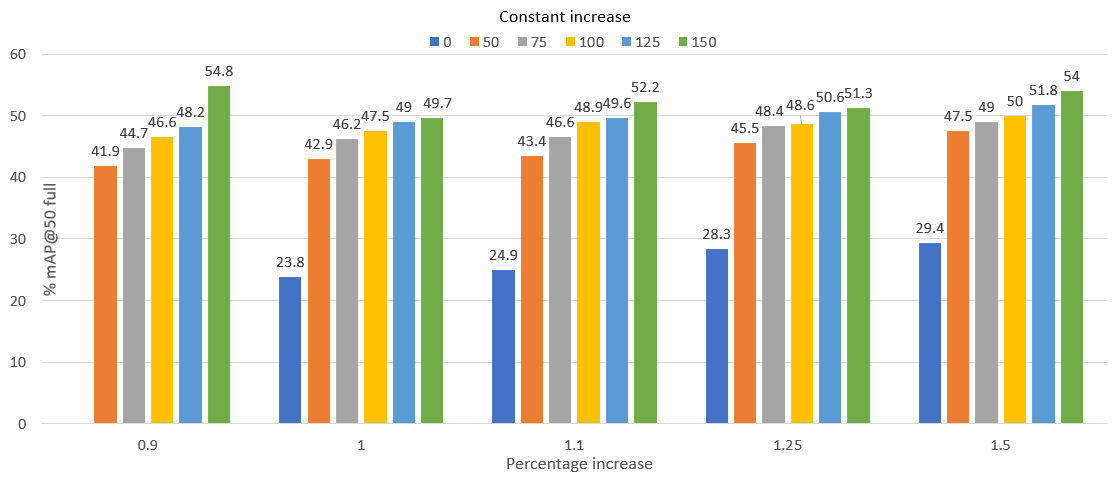
\includegraphics[scale=0.6]{figures/SwitchPreprocess.png}}
	\caption{Comparison between combinations of fixed and percentage-based switch enlargement based on mAP@50 full.\\
    \textcolor{green}{oare daca ai pune pe axa Ox cresterile cantitative si cu culori sa diferentiezi modificarile procentuale nu s-ar alinia mai bine cu explicatia din text?\\ \textcolor{red}{Ar fi mai bine asa, voi reface graficul.}
    In plus, in tabele valorile pt mAP sunt date pe scara (0,1), aici, in figura, sunt pe scara (0, 100); ar fi bine sa se foloseasca aceeasi scara \textcolor{red}{Nu incapeau in grafic in varianta (0,1). Voi mofica sa fie uniform.}
    }
 }
	\label{fig:switch_enlargement_exp}
\end{figure*}

These increases in detection performance are obtained while also performing rail guard semantic segmentation. The results for the semantic segmentation can bee seen in the following table, \textbf{Table \ref{tab:exp_uolo_seg_railsem19_subsets}}. Surprisingly, the segmentation which can exploit all images, no matter the presence of switches, is not improved by a larger subset. There seems to be a strong relationship between the two objectives, which is to be expected as they share a large amount of the combined neural network. 


The best performance is achieved when the images with no switches are eliminated. Further investigation shows that the limitations from the semi-supervised semantic annotation process are most prevalent in those images. As the automatic part of the labeling process is conducted based on guidance inferred from the object detection annotations, the images with no switches have semantic labels of worse quality. The most extreme scenario in which the dataset has to suffer is when the guard rails annotation is completely missing. Using images in which at least one switch is present helps us address this issue to a certain extent, explaining the drastic increase in performance. From this point forward we continue our experiments on the subset with no unknown switches and no images containing no switches for two reasons. First of all, the filtering of the unknown class allows us to also evaluate the classification capabilities of our network. We also filter out the images with no switches as they contain far more mistakes in their semantic segmentation annotations.

\begin{table}[ht]
    \centering
    \caption{\textcolor{red}{UOLO} performance on RailSem19 subsets.
    \textcolor{green}{\\sunt rezultate obtinute cu YoloV5 sau cu UOLO? in text se spune ca sunt obtinute cu UOLO.\textcolor{red}{Cu UOLO.}}
    }
    \begin{tabular}{cccc}
    \hline
   \begin{tabular}{@{}c@{}}\textbf{Unknown switches} \\ \textbf{No switches} \end{tabular} & \textbf{No. images} & \textbf{mean IoU} & \textbf{rail IoU} \\
     \hline\hline
     \begin{tabular}{@{}c@{}}Yes\\ Yes\end{tabular} & 8500 & 0.613 & 0.265 \\ 
     \hline
     \begin{tabular}{@{}c@{}}Yes\\ No\end{tabular} & 6976 & 0.696 & 0.42 \\
     \hline
     \begin{tabular}{@{}c@{}}No\\ Yes\end{tabular} & 2764 & 0.551 & 0.145 \\ 
     \hline
     \begin{tabular}{@{}c@{}} No\\ No\end{tabular} & 1240 & 0.683 & 0.393 \\
     \hline
    \end{tabular}
    \label{tab:exp_uolo_seg_railsem19_subsets}
\end{table}

After this initial experiment which showcased the potential of multi-task learning, we focus our attention on preprocessing the switches. We enlarge the initial annotation in order to capture further information which should facilitate the detection performance. The positive impact should be even greater for the classification task, in which the supplementary context is absolutely necessary, as without the blades there is no distinguishable characteristic in switches. 

In \textbf{Fig. \ref{fig:switch_enlargement_exp}}, a comparison between the enlargement values can be observed, based on the mAP@50 performance on both the detection and classification. In most cases, as the enlargement increases the performance is also improved. The only combinations of fixed and percentage-based increase we do not experiment with is the one with no constant increase in which the dimensions would be multiplied by 0.9. We made the choice to omit this combinations as it defeats the purpose of enlarging bounding boxes. The remaining results obtained by combining this percentage-based reduction with constant increases suggest it has no beneficial effect until a larger fixed increase like 150 is used. For that pair, the best mAP@50 full value is obtained, specifically 54.8\%. 

\begin{table}[ht]
    \centering
    \caption{Impact of the geometric preprocessing. \textcolor{red}{Model trained on images containing only left and right switches}\\
    \textcolor{green}{1. nu ar merita adaugata mean IoU pt switches?\\ 
    \textcolor{red}{Intr-un fel mean IoU-ul pt switches e parte din mAP, dar se poate adauga ca sa fie completa analiza}
    2. tb reamintit scenariul in care esti, corespunzator imaginilor folosite (left + right?)}
    }
    \begin{tabular}{ccccc}
    \hline
   \begin{tabular}{@{}c@{}}\textbf{Geometric} \\ \textbf{Preprocess} \end{tabular} & \textbf{mean IoU} & \textbf{rail IoU} & \textbf{mAP det} & \textbf{mAP full} \\
     \hline\hline
      No & 0.693 & 0.412 & 0.862 & 0.513 \\ 
     \hline
     Yes & 0.812 & 0.606 & 0.870 & 0.514 \\
     \hline
    \end{tabular}
    \label{tab:geometric_preprocess}
\end{table}

As the extra input channels offers a first segmentation mask which requires refinement, the most noticeable impact of this technique is seen in the mean IoU obtained by the segmentation path, whose performance is increased by more than 10\% IoU, as observed in \textbf{Table \ref{tab:geometric_preprocess}}. When it comes to the rail IoU the previous value, 0.412 rises to 0.606.  The performance of detection and classification is also slightly increased. 

\textcolor{green}{experimentul urmator nu mai are treaba cu switch-urile, asa-i? e vorba doar despre sine si, pt a putea compara rezultatele cu RailCNN, scopul segmentarii e predictia rail-track-urilor?}
\textcolor{red}{Modelul e antrenat tot in mod multitask: switch detection + rail track segmentation, dar intradevar detectia macazului e un aspect secundar aici.}

We also run an experiment in which instead of segmenting the guard-rail we extract the rail-track. In this task we achieve a mean IoU of 93.5\%, exceeding the previous best performance achieved by RailCNN 
\textcolor{green}{add a ref} \textcolor{red}{\cite{belyaev2020railroad}}
by 0.4\%, 
\textcolor{green}{\\1. adica cu RailCNN s-a obtinut un meanIou de 93.1?\\ 
2. atentie la scara valorilor (0,100) sau (0,1). Oricare e ok, dar ideea e sa fie peste tot la fel (in text, in tabele, in figuri)\\}
\textcolor{red}{1. Da \\2. Voi modifica sa fie la fel}
on smaller images while also performing detection. The proposed approach is also competitive in guard-rail semantic segmentation, a task in which we outperform the best reported performance by 0.2\%, while respecting real-time constraints. In switch detection, we are able to obtain up to 87\% mAP an impressive value for the RailSem19 dataset, on which due to limitations in annotation no other notable model was proposed. On other private datasets, RetinaNet \cite{jahan2021deep} reaches over 95\%, but we are unable to test our approach on this data. Lastly, the limitation of this multitask approach is the classification which does not exceed 66\%. This weakness suggests, that at least at the moment the task requires a specialized network

\subsection{re-organizare}
\textcolor{green}{eu as propune o mica re-organizare a experimentelor ca sa fie mai usor de urmarit. O sa scriu cu negru ca sa imi fie mai usor}

Ideea e asa: eu am identificat 3 thread-uri mari in aceste experimente:
\begin{itemize}
    \item switch identification in raw images; 
    \item switch identification in pre-processed images; 
    \item guard-rail and rail-track identification.
\end{itemize}

Ca sa fie mai usor as da detaliile legate de dataset distribution si metricile de performanta inainte de inceperea descrierii experimentelor. Adica:
\begin{itemize}
    \item Sectiunea 4.1 - descrierea datasetului (ceea ce e acum)
    \item Sectiunea 4.2 - prerequisites 
    \begin{itemize}
        \item descrierea subseturilor folosite in experimente
            \begin{itemize}
                \item pt switch identification as include un tabel de forma
                    \begin{table}[]
                        \centering
                        \caption{Data distribution}
                        \begin{tabular}{c|c|c}
                             Type           & \# images & \# instances \\ \hline
                             left switch    & x         & a \\ \hline
                             right switch   & y         & b \\ \hline
                             unknown switch & z         & c \\ \hline
                             no switch      & t         & d \\ \hline
                        \end{tabular}                        
                        \label{tab:dataDistribution}
                    \end{table}
                \item apoi as definiti scenariile mentionate in tabelele cu rezultatele. De exemplu:
                    \begin{itemize}
                        \item $Scenario_1$ = x+ y + z + t corespunde la prima linie din tabelele \ref{tab:exp_yolov5_railsem19_subsets} si \ref{tab:exp_uolo_railsem19_subsets}
                        \item $Scenario_2$ = x+ y + z corespunde la a 2-a linie din tabelele \ref{tab:exp_yolov5_railsem19_subsets} si \ref{tab:exp_uolo_railsem19_subsets}
                        \item + celelalte 2 scenarii
                    \end{itemize}
                \item as descrie similar si subseturile folosite pt guard-rail si rail-track identification
            \end{itemize}   
        \item descrierea metricilor (mAP@50 det, mAP@50 full, mean IoU). As zice o propozitie despre ce reprezinta fiecare + referinta, apoi prima parte din al 2-lea paragraf al sectiunii IV.B
    \end{itemize}
    \item Sectiunea 4.3 - numerical experiments - pe care le-as prezenta in ordinea si structurarea urmatoare:
        \begin{itemize}
            \item Experiment 1 - switch identification (by YoloV5 and UOLO) in raw images (aici ar intra paragraful 1 din IV.B, a 2-a parte din paragraful 2 din  (aici ar intra IV.B, paragraful 3 din IV.B
                \begin{itemize}
                    \item Aim - inspect the capability of UOLO vs other detectors from the literature
                    \item data - raw images form Scenario 1/2/3/4
                    \item models - different detectors and UOLO
                    \item results and discussion - tables \ref{tab:exp_yolov5_railsem19_subsets} si \ref{tab:exp_uolo_railsem19_subsets}
                \end{itemize}
            \item Experiment 2 - switch identification (by UOLO) in pre-processed images (aici ar intra paragrafele 6,7,8 in IV.B)
                \begin{itemize}
                    \item Aim - analyse the impact of a supplementary channel in the uOLO's input
                    \item data - pre-processed images form Scenario 3? (x + y?)
                    \item models - UOLO + channel-ul suplimentar care suplimenteaza inputul cu pre-procesarile
                    \item results and discussion - table \ref{tab:geometric_preprocess}, figure \ref{fig:switch_enlargement_exp}
                \end{itemize}
            \item Experiment 3 - guard-rail identification (aici ar intra paragraful 4,5 din IV.B)
                \begin{itemize}
                    \item Aim - versatility (or genralisation ability) of UOLO for other objects (not only switches)
                    \item data - images from Scenario 6? (no of images / instances for every class used in this experiment); raw or pre-processed?
                    \item models - UOLO simplu sau UOLO + channel-ul suplimentar care suplimenteaza inputul cu pre-procesarile
                    \item results and discussion - table \ref{tab:exp_uolo_seg_railsem19_subsets}
                \end{itemize}
              \item Experiment 4 - rail-track identification (aici ar intra paragraful 9 (ultimul) din IV.B) 
                \begin{itemize}
                    \item Aim - versatility (or genralisation ability) of UOLO for other objects (not only switches) - the selection of the object is driven by the possibility to compare to other models from the literature
                    \item data - images from Scenario 7? (no of images / instances for every class used in this experiment); raw or pre-processed?
                    \item models - UOLO simplu sau UOLO + channel-ul suplimentar care suplimenteaza inputul cu pre-procesarile, RailCNN
                    \item results and discussion - those from text
                \end{itemize}
            \item e posibil si sa se reuneasca exp 3 si exp 4 intr-unul singur 
            \item De adaugat o subsectiune / un paragraf care sa rezume imbunatatirile obtinute si sa se evidentieze raspunsuri la cele 2 RQs din finalul Introducerii. De asemenea, pot fi incluse cateva threats-uri ale analizelor efectuate; de ex.: un singur set de date - chiar daca nu exista alt set public, testarea doar pe un set de imagini e un punct slab; trade-off-ul dintre performanta si efortul computational.
        \end{itemize}
\end{itemize}
\end{comment}
\fi

\section{Conclusions and Future Considerations}
\label{conclusion}

In this article, an efficient real-time robust solution was proposed for guard-rail semantic segmentation and switch detection. The method showcases the benefits of both multi-task learning and classic computer vision algorithms, which when fused with deep learning can drastically increase the performance of models in rail scene understanding. 

UOLO is able to achieve impressive results, outperforming all existing approaches in three out of the four tackled tasks: switch detection, track semantic segmentation and rail semantic segmentation. The applicability of the model when used by itself is still limited by the poor classification performance, but the FPS of the approach which is over 22 would allow the combination with a light-weight dedicated classifier.

We strive to continue the improvement of our approach in the following ways.
\begin{itemize}
    \item Modify the classification head of the UOLO model in order to make it more suitable for the switch classification task
    \item Further test the generality of the model on related datasets which contain rail annotations like Cityscapes 
    \item Apply hyper-parameter search in order to improve the computation of the geometric prior
\end{itemize}

\section{Acknowledgements}
\label{acknowledgements}

This work was supported by Babe\c{s}-Bolyai University, through scientific scholarship 36596 / 25 nov 2022. 

\balance

\printbibliography

\vspace*{1\baselineskip}

\textbf{Alexandru Manole} received the master’s degree in applied computational intelligence from the Babe\c{s}-Bolyai University in 2023. During his studies, he was part of multiple Computer Vision research projects, two of them focusing on intelligent solutions for rail transportation.

\vspace*{1\baselineskip}

\textbf{Laura Dioșan} is currently full professor in the Department of Computer Science at UBB. She has a vast research experience participating in more than ten projects in the last 15 years, from which she coordinated three projects successfully completed. Her research areas cover evolutionary optimisation, swarm intelligence and machine learning with excellent research results obtained by different hybrid models given by evolutionary computation and kernel algorithms for image processing and classification. Another part of her research activity has been dedicated to self-adaptation of algorithms to the problem to be solved (in order to improve the quality of the solving/learning process) through the parameter optimisation and through the fusion of information. Research results have been published in journals and conference papers obtaining more than 300 citations.


\end{document}